\documentclass[aspectratio=169, 12pt, hyperref={unicode}]{beamer}
\usepackage[utf8]{inputenc}
\usepackage[czech]{babel}
\usepackage{graphicx}
\usetheme{Madrid}
\usepackage{times}
\usepackage{lipsum}
\usepackage{subcaption}

\usepackage[euler]{textgreek}
\usepackage[font=footnotesize]{caption}


\title{Měření úniků mobilního spoje}
\subtitle{B2M17SBS -- Projekt II}
\author{Šimák, Hulec, Semerád, Jína}
\date{Květen 2023}


\definecolor{cvut_navy}{HTML}{0065BD}
\definecolor{cvut_blue}{HTML}{6AADE4}
\definecolor{cvut_gray}{HTML}{156570}

\setbeamercolor{section in toc}{fg=black,bg=white}
\setbeamercolor{alerted text}{fg=cvut_blue}
\setbeamercolor*{palette primary}{bg=cvut_navy,fg=gray!20!white}
\setbeamercolor*{palette secondary}{bg=cvut_blue,fg=white}
\setbeamercolor*{palette tertiary}{parent=palette primary}
\setbeamercolor*{palette quaternary}{fg=green,bg=gray!5!white}

\setbeamercolor*{sidebar}{fg=cvut_navy,bg=gray!15!white}


\setbeamercolor{titlelike}{parent=palette primary}
\setbeamercolor{frametitle}{parent=palette primary}

\setbeamercolor*{separation line}{}
\setbeamercolor*{fine separation line}{}

\setbeamertemplate{navigation symbols}{} 

\setbeamercolor{itemize item}{fg=cvut_blue}
\setbeamercolor{itemize subitem}{fg=cvut_blue}
\setbeamercolor{itemize subsubitem}{fg=cvut_blue}
\setbeamercolor{section number projected}{bg=cvut_navy}
\setbeamercolor{caption name}{fg=cvut_blue}

\setbeamertemplate{itemize item}[circle]
\setbeamertemplate{itemize subitem}[circle]
\setbeamertemplate{itemize subsubitem}[circle]
\setbeamertemplate{caption}[numbered]


\begin{document}

\logo{
\includegraphics[height=1cm]{src/symbol_cvut_plna_samostatna_verze.pdf}}

\begin{frame}
	\titlepage
\end{frame}

\begin{frame}
	\frametitle{Obsah}
	\tableofcontents
\end{frame}

\section{Zadání}
	\begin{frame}
	\frametitle{Zadání - cíle}
	\begin{itemize}
		\item Realizovat měření v terénu v pásmu UHF (200~MHz až 3~GHz) za účelem lepšího porozumění podstatě úniků mobilního spoje
		\item Využít měřená data pro odvození empirického modelu závislosti ztrát na vzdálenosti.
		\item Na základě výsledků měření statisticky analyzovat úniky způsobené vícecestným šířením.
	\end{itemize}
	\vspace*{5pt}
	\textbf{Scénář měření:} venkovní prostředí uvnitř husté městské zástavby\\
	\textbf{Frekvence:} 2,7~Ghz
	\end{frame}

	\begin{frame}
	\frametitle{Zadání - použité vybavení}
	\begin{itemize}
		\item přenosný UHF generátor
		\item přenosný přijímač Rohde \& Schwarz PR100
		\item $2\times$ všesměrová anténa se stojanem
		\item pásmo na měření vzdálenosti, výšky antén apod.
		\item fotoaparát či mobilní telefon pro dokumentaci měření
	\end{itemize}
	\end{frame}

\section{Měření I - Empirický model}
\subsection{Jugoslávských partyzánů}
\begin{frame}{Jugoslávských partyzánů}
	\begin{figure}[!ht]
		\centering
		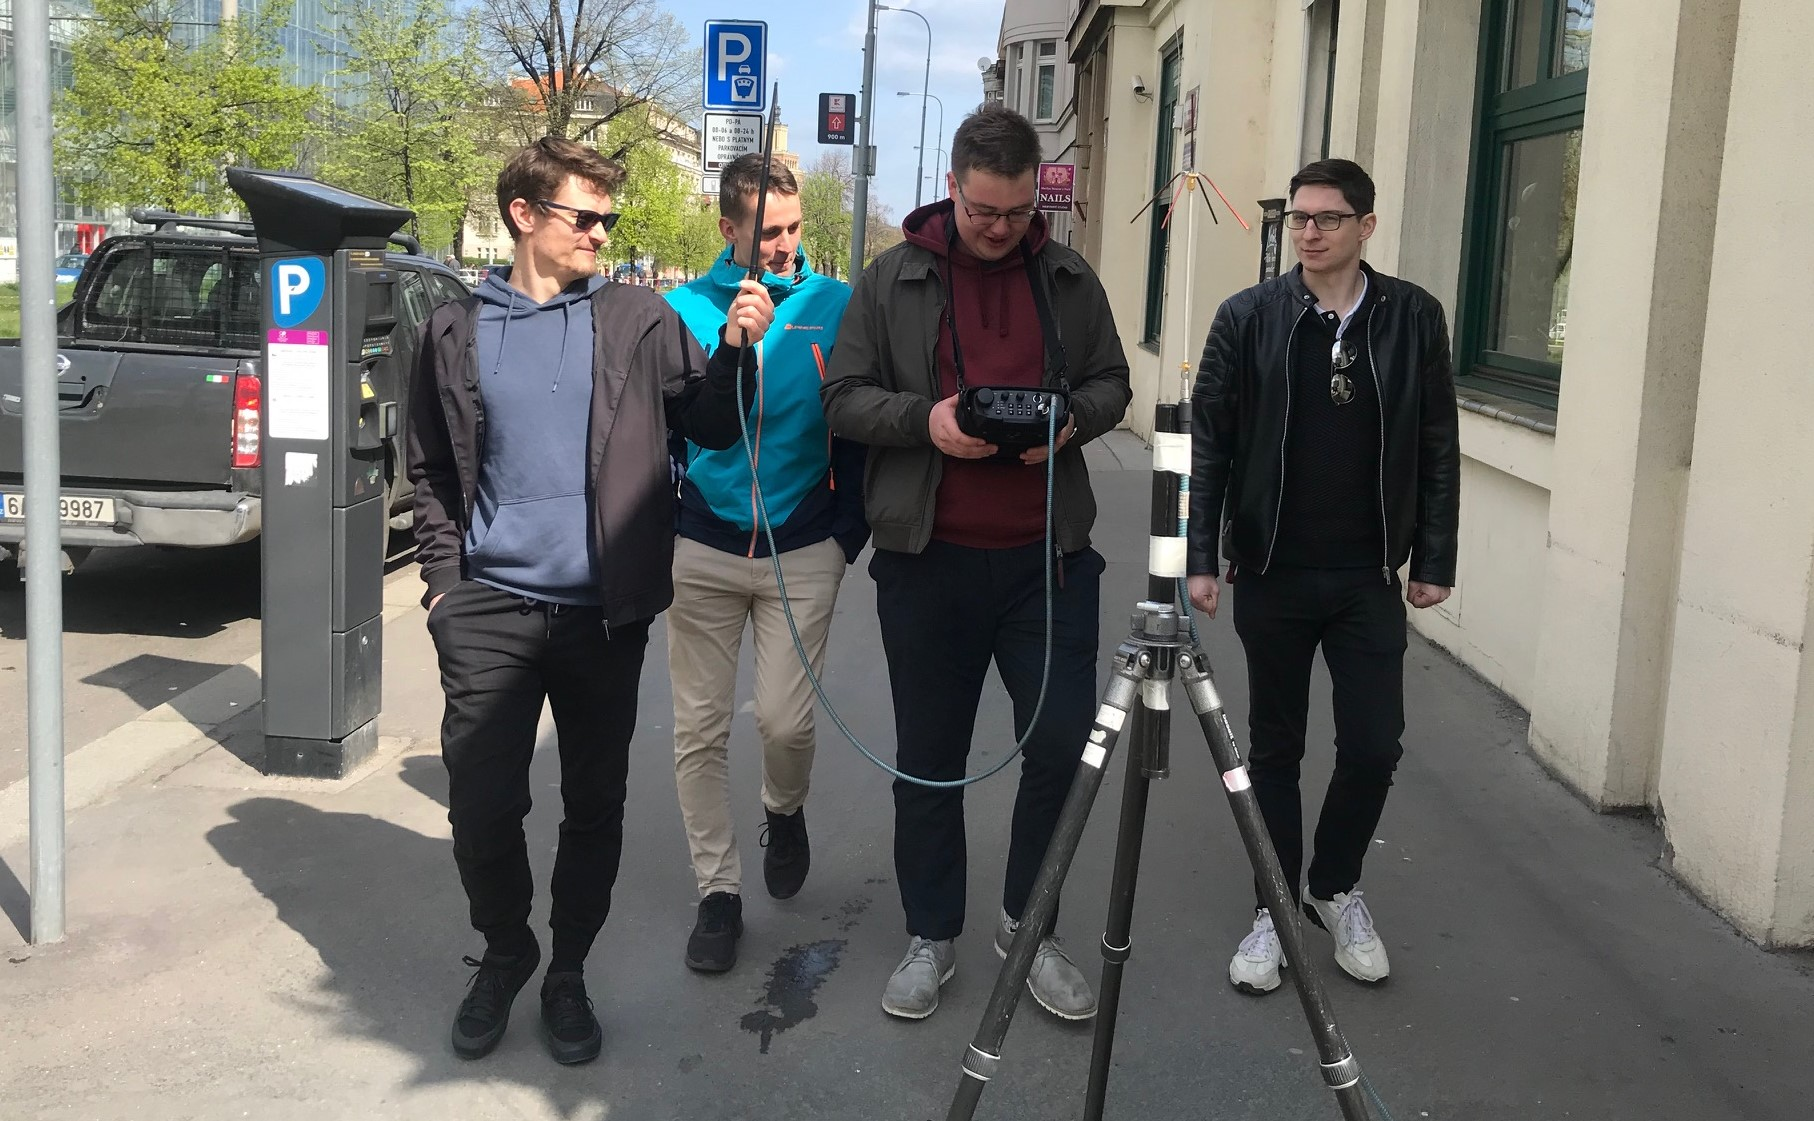
\includegraphics[width=.7\textwidth]{src/fotka-skupina.jpg}
	\end{figure}
\end{frame}
\begin{frame}{Jugoslávských partyzánů - cesta od vysílače}
	\begin{figure}[!ht]
		\centering
		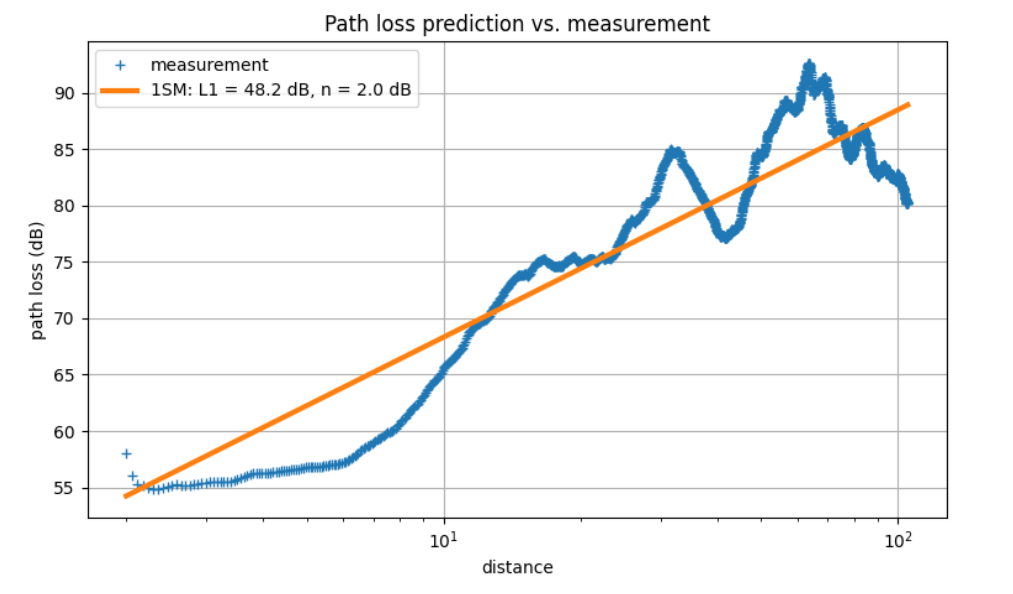
\includegraphics[width=.75\textwidth]{src/partyzanu-od-vysilace-1.png}
	\end{figure}
\end{frame}
\begin{frame}{Jugoslávských partyzánů - cesta od vysílače}
	\begin{figure}[!ht]
		\centering
		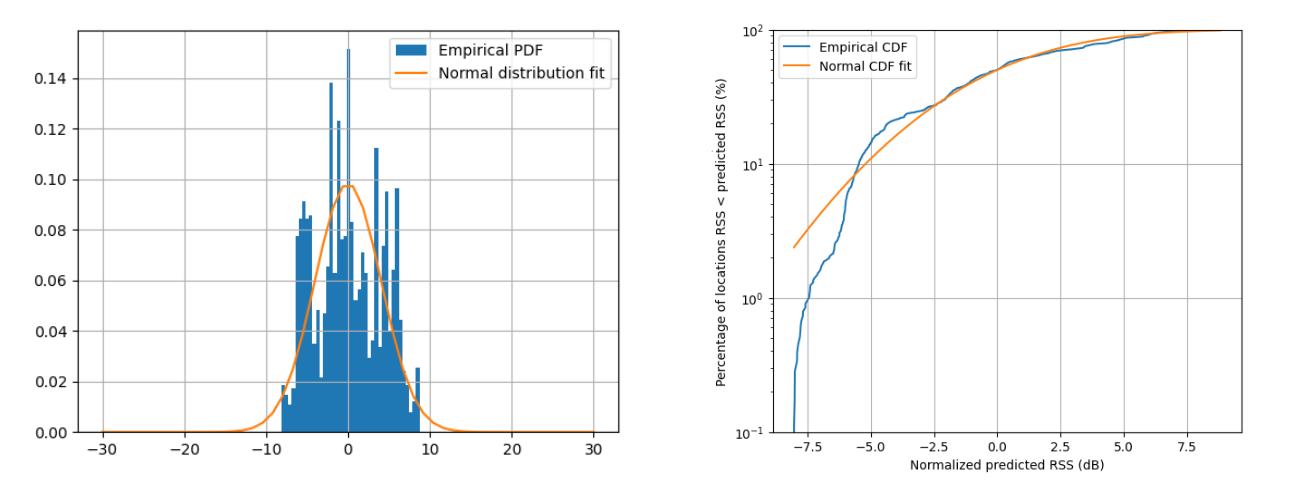
\includegraphics[width=\textwidth]{src/partyzanu-od-vysilace-2.png}
	\end{figure}
\end{frame}
\begin{frame}{Jugoslávských partyzánů - cesta od vysílače}
	\begin{figure}[!ht]
		\centering
		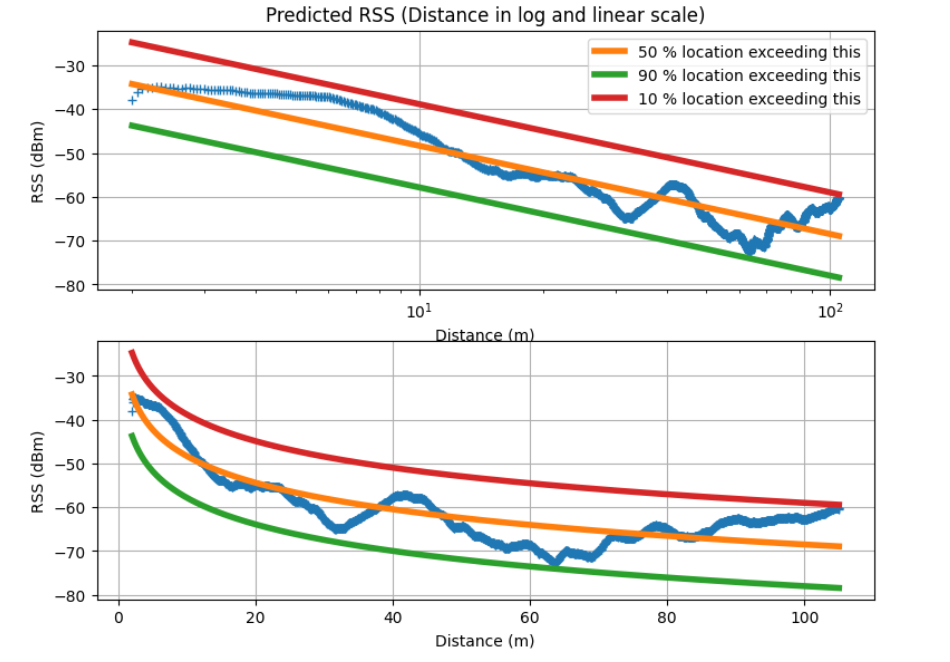
\includegraphics[width=.6\textwidth]{src/partyzanu-od-vysilace-3.png}
	\end{figure}
\end{frame}
\begin{frame}{Jugoslávských partyzánů - cesta k vysílači}
	\begin{figure}[!ht]
		\centering
		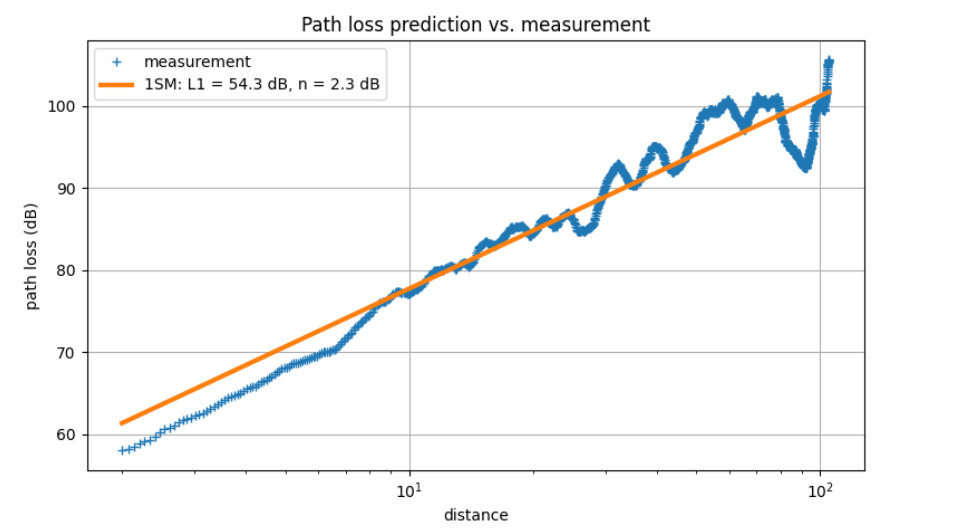
\includegraphics[width=.75\textwidth]{src/partyzanu-k-vysilaci-1.png}
	\end{figure}
\end{frame}
\begin{frame}{Jugoslávských partyzánů - cesta k vysílači}
	\begin{figure}[!ht]
		\centering
		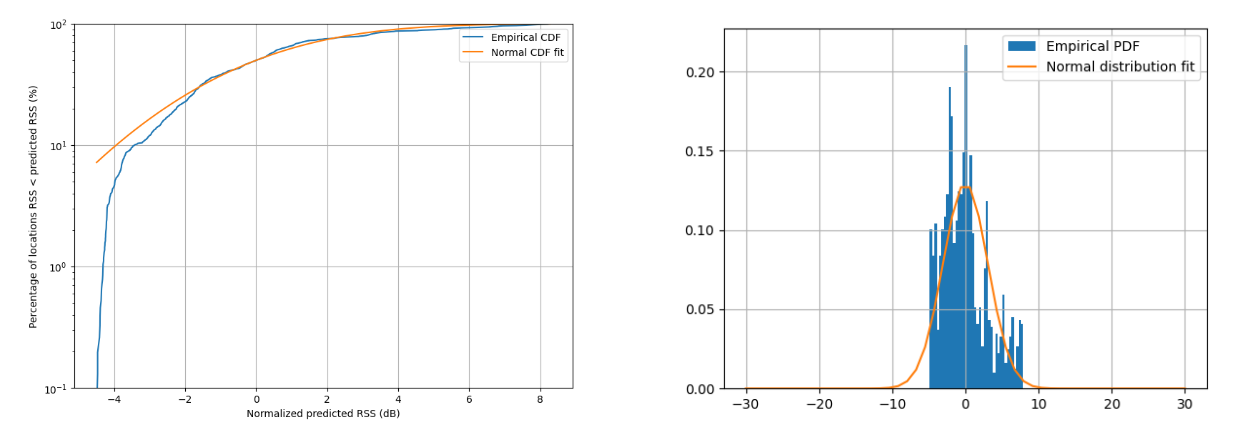
\includegraphics[width=\textwidth]{src/partyzanu-k-vysilaci-2.png}
	\end{figure}
\end{frame}
\begin{frame}{Jugoslávských partyzánů - cesta k vysílači}
	\begin{figure}[!ht]
		\centering
		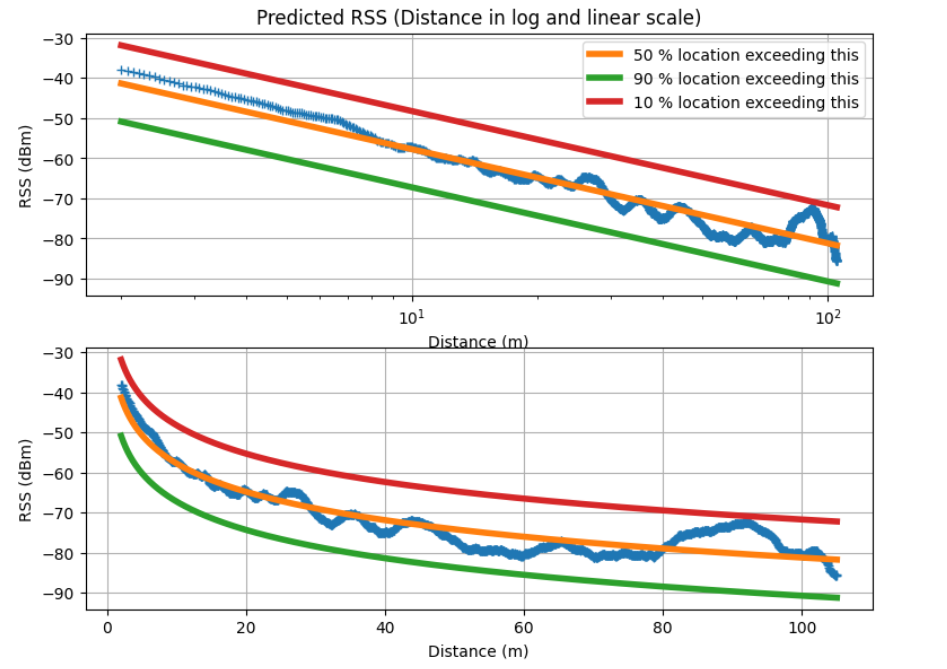
\includegraphics[width=.6\textwidth]{src/partyzanu-k-vysilaci-3.png}
	\end{figure}
\end{frame}

\subsection{Terronská}
\begin{frame}{Terronská}
	\begin{figure}[!ht]
		\centering
		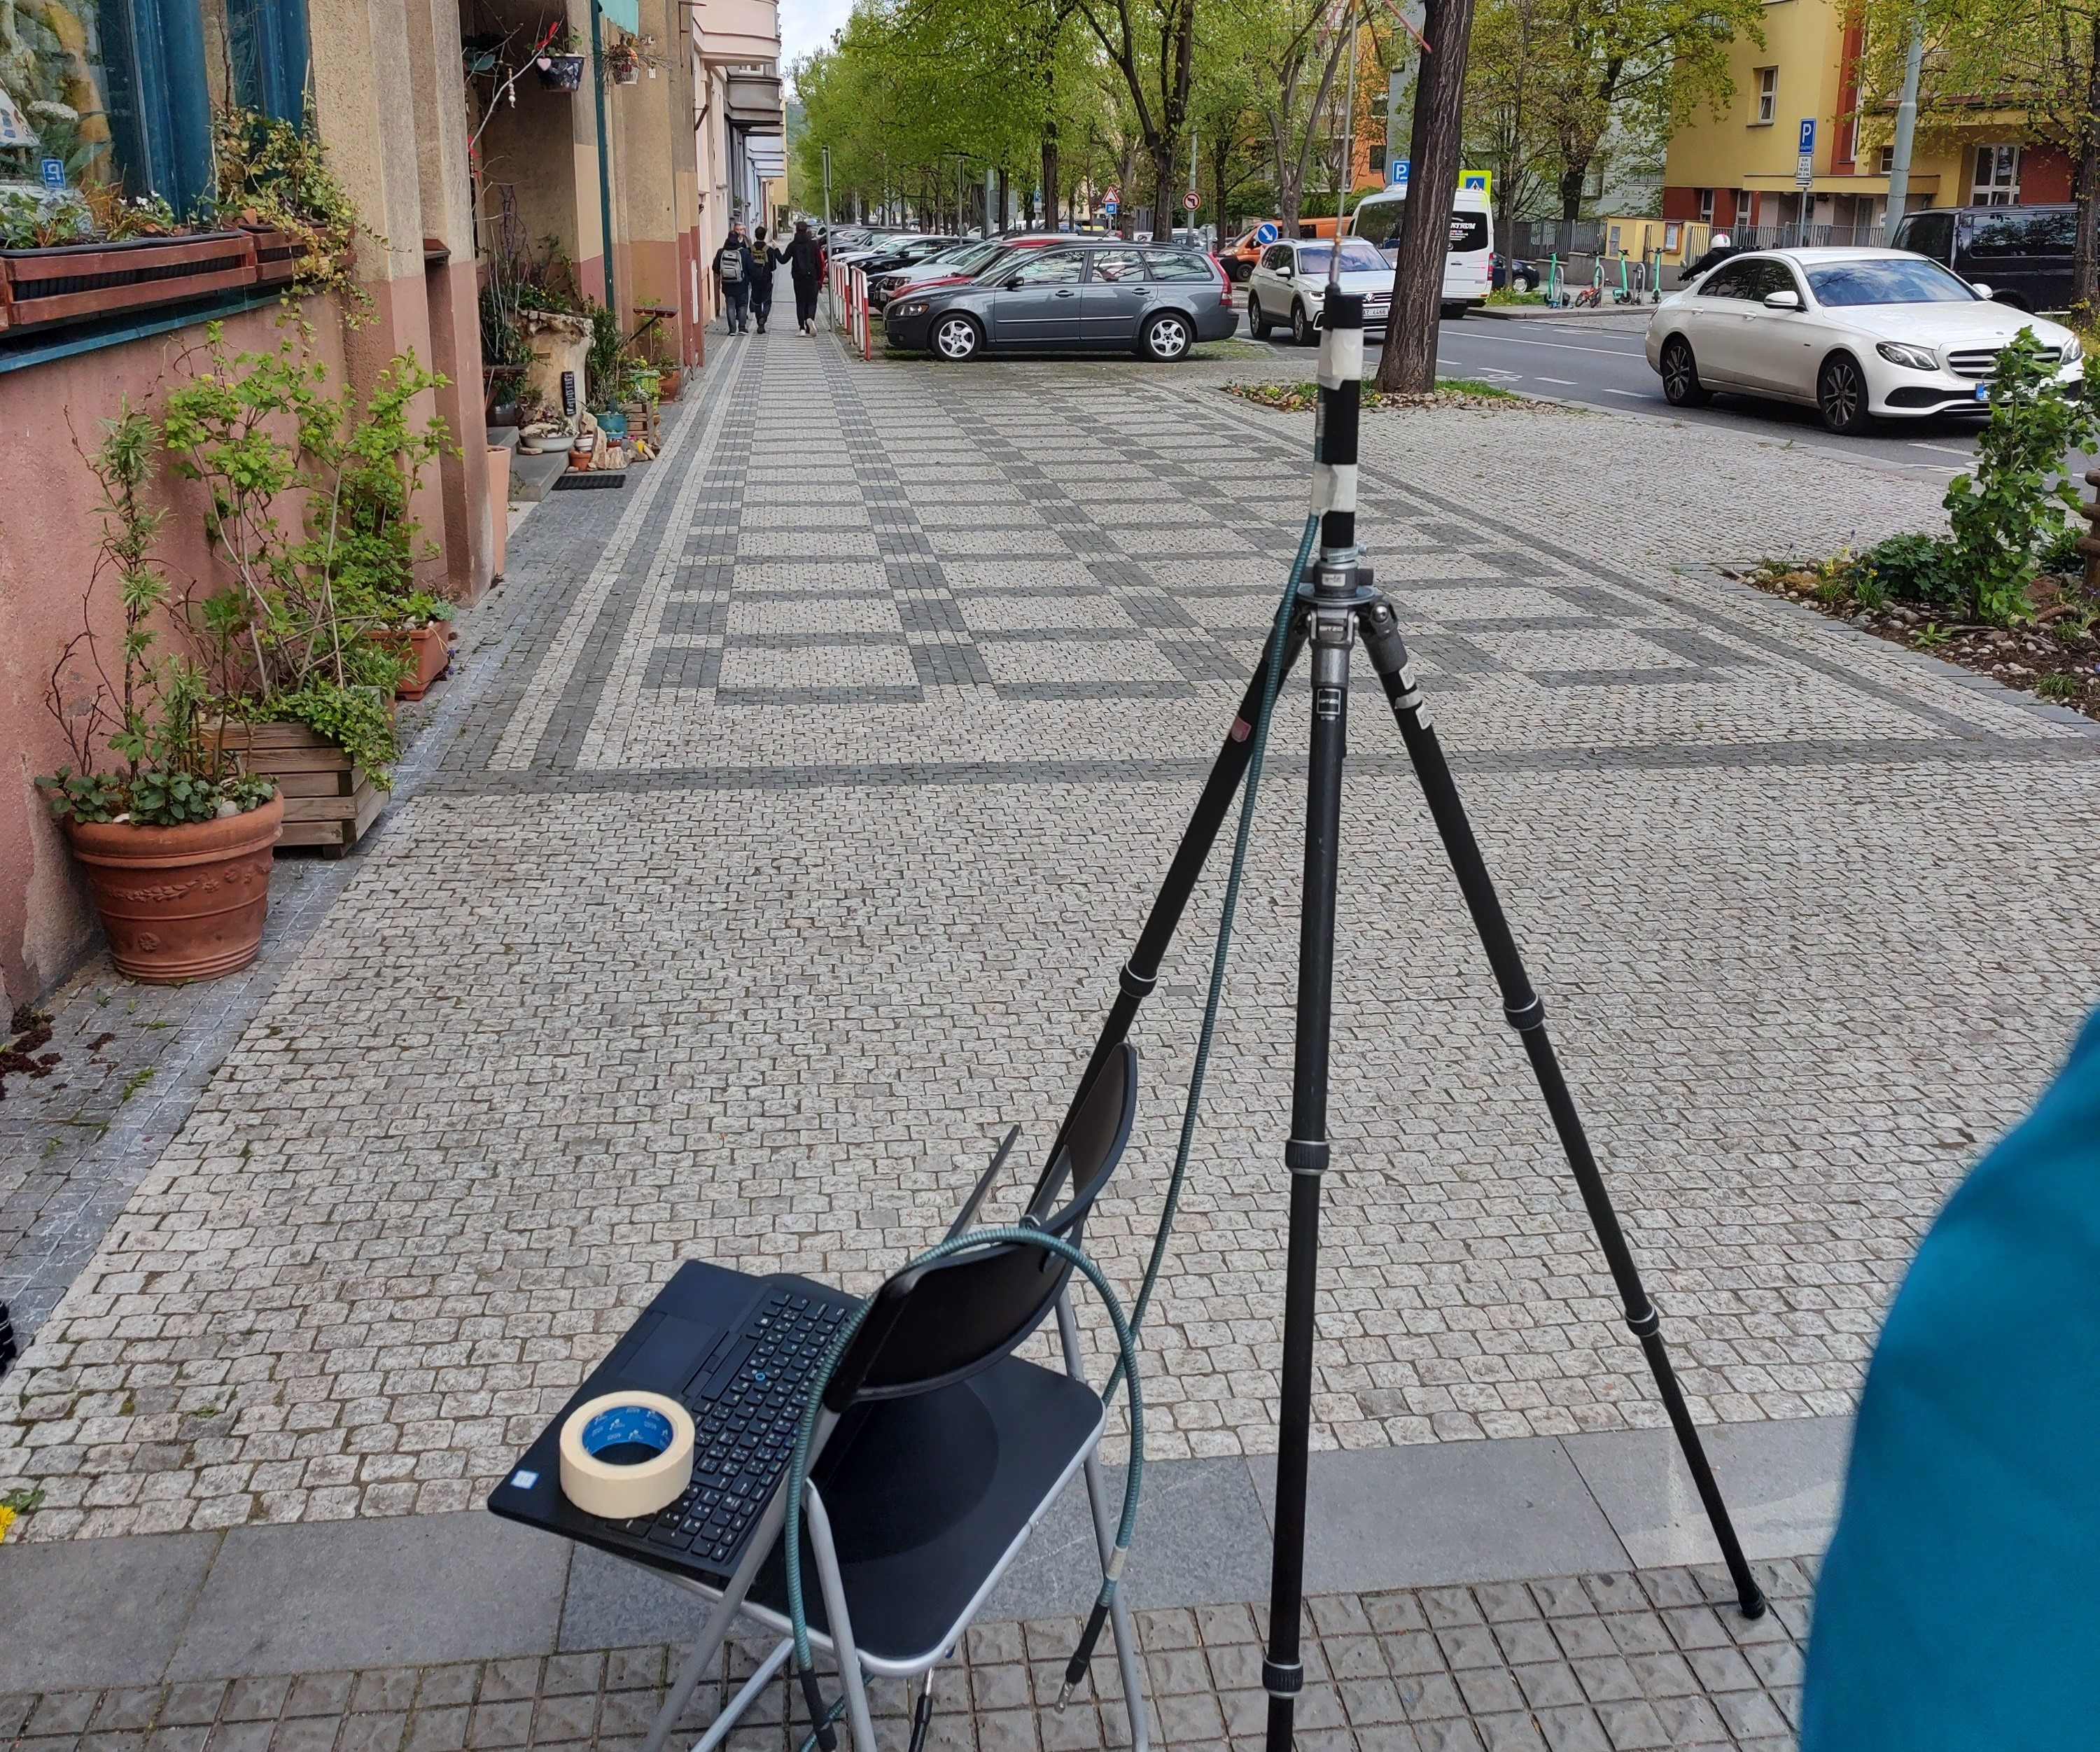
\includegraphics[angle=0,width=.5\textwidth]{src/fotka-terronska.jpg}
	\end{figure}
\end{frame}
\begin{frame}{Terronská - cesta od vysílače}
	\begin{figure}[!ht]
		\centering
		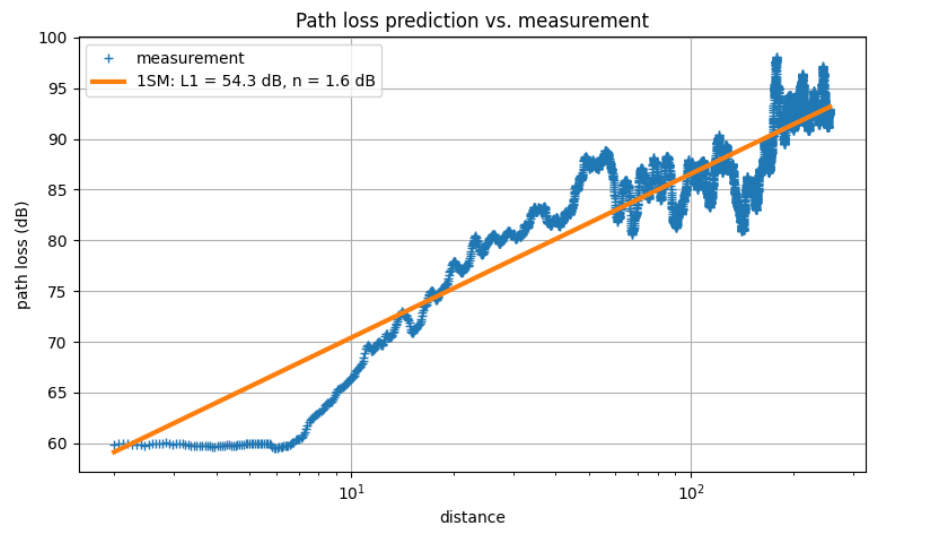
\includegraphics[width=.75\textwidth]{src/terronska-od-vysilace-1.png}
	\end{figure}
\end{frame}
\begin{frame}{Terronská - cesta od vysílače}
	\begin{figure}[!ht]
		\centering
		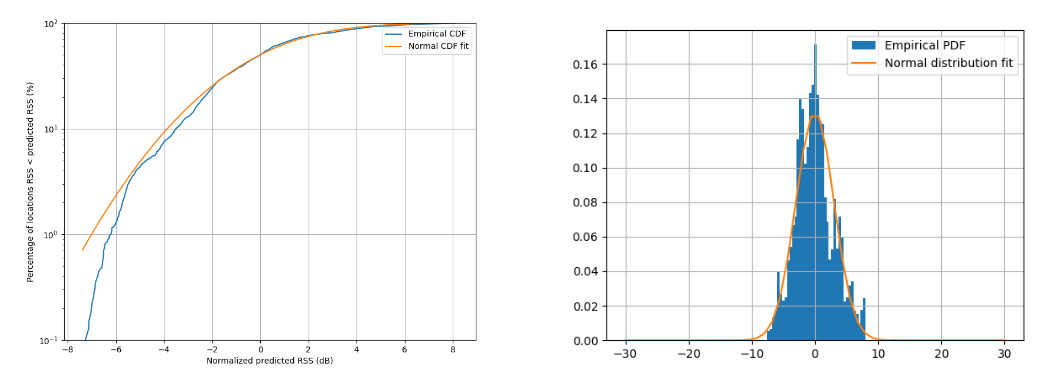
\includegraphics[width=.95\textwidth]{src/terronska-od-vysilace-2.png}
	\end{figure}
\end{frame}
\begin{frame}{Terronská - cesta od vysílače}
	\begin{figure}[!ht]
		\centering
		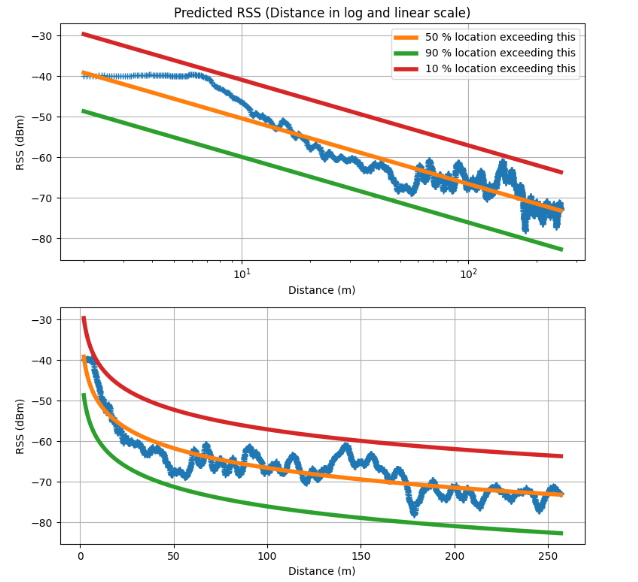
\includegraphics[width=.5\textwidth]{src/terronska-od-vysilace-3.png}
	\end{figure}
\end{frame}
\begin{frame}{Terronská - cesta k vysílači}
	\begin{figure}[!ht]
		\centering
		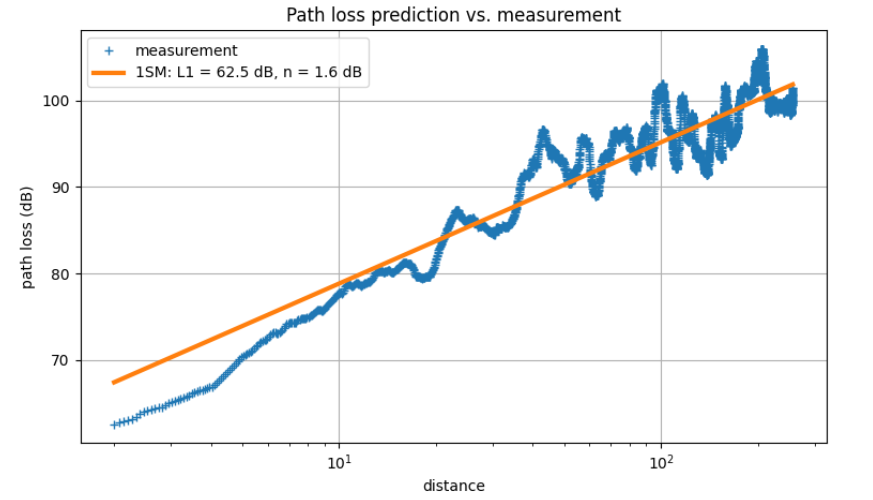
\includegraphics[width=.75\textwidth]{src/terronska-k-vysilaci-1.png}
	\end{figure}
\end{frame}
\begin{frame}{Terronská - cesta k vysílači}
	\begin{figure}[!ht]
		\centering
		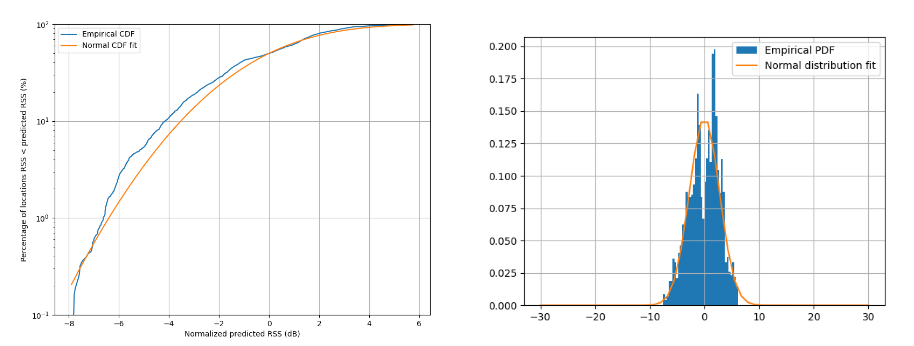
\includegraphics[width=.9\textwidth]{src/terronska-k-vysilaci-2.png}
	\end{figure}
\end{frame}
\begin{frame}{Terronská - cesta k vysílači}
	\begin{figure}[!ht]
		\centering
		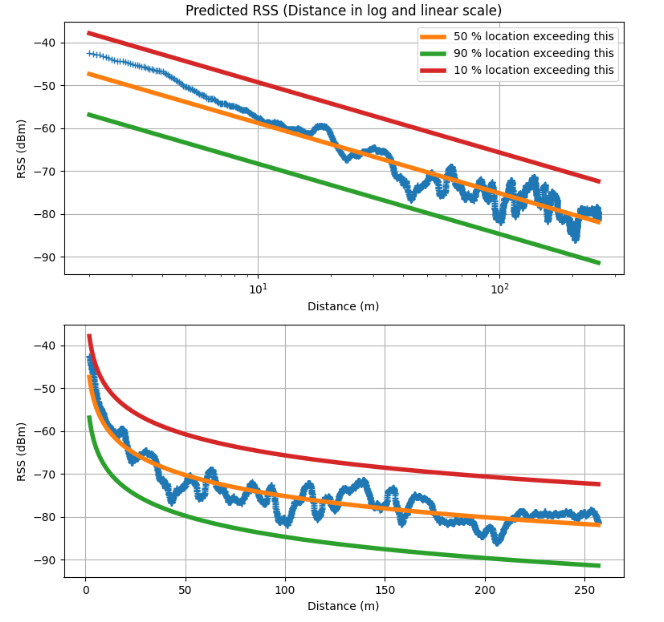
\includegraphics[width=.5\textwidth]{src/terronska-k-vysilaci-3.png}
	\end{figure}
\end{frame}

\section{Měření II - Úniky způsobené vícecestným šířením}
\begin{frame}{Úniky - naměřené výkony}
	\begin{figure}[!ht]
		\centering
		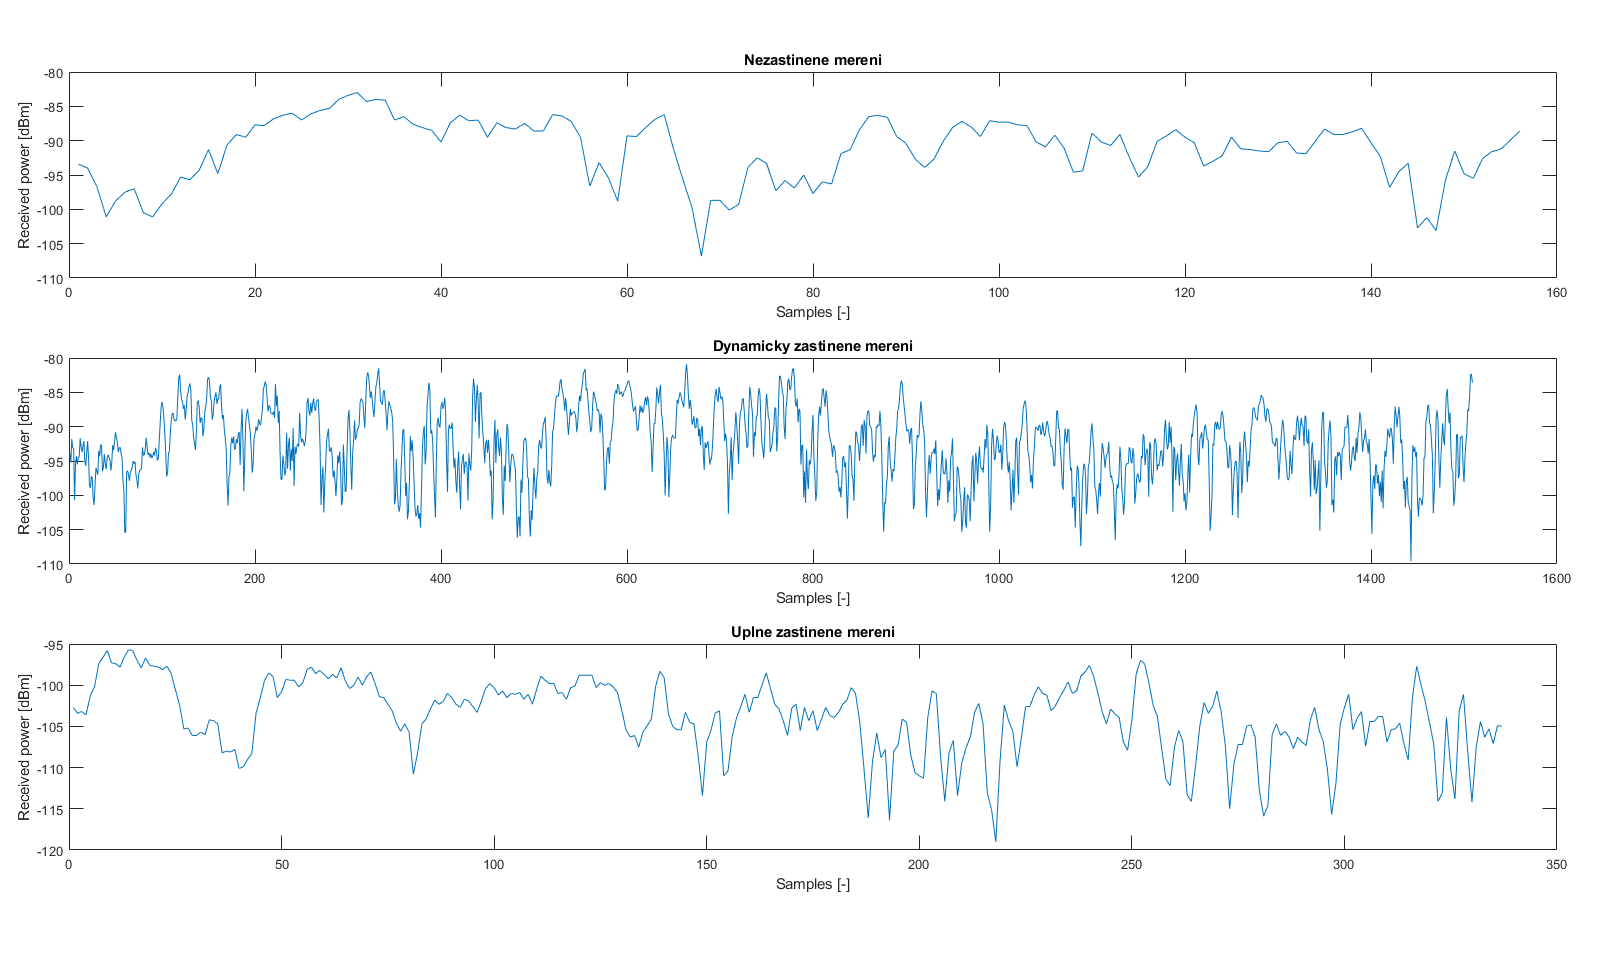
\includegraphics[width=.75\textwidth]{src/uniky-vykon.png}
	\end{figure}
\end{frame}
\begin{frame}{Úniky - CDF}
	\begin{figure}[!ht]
		\centering
		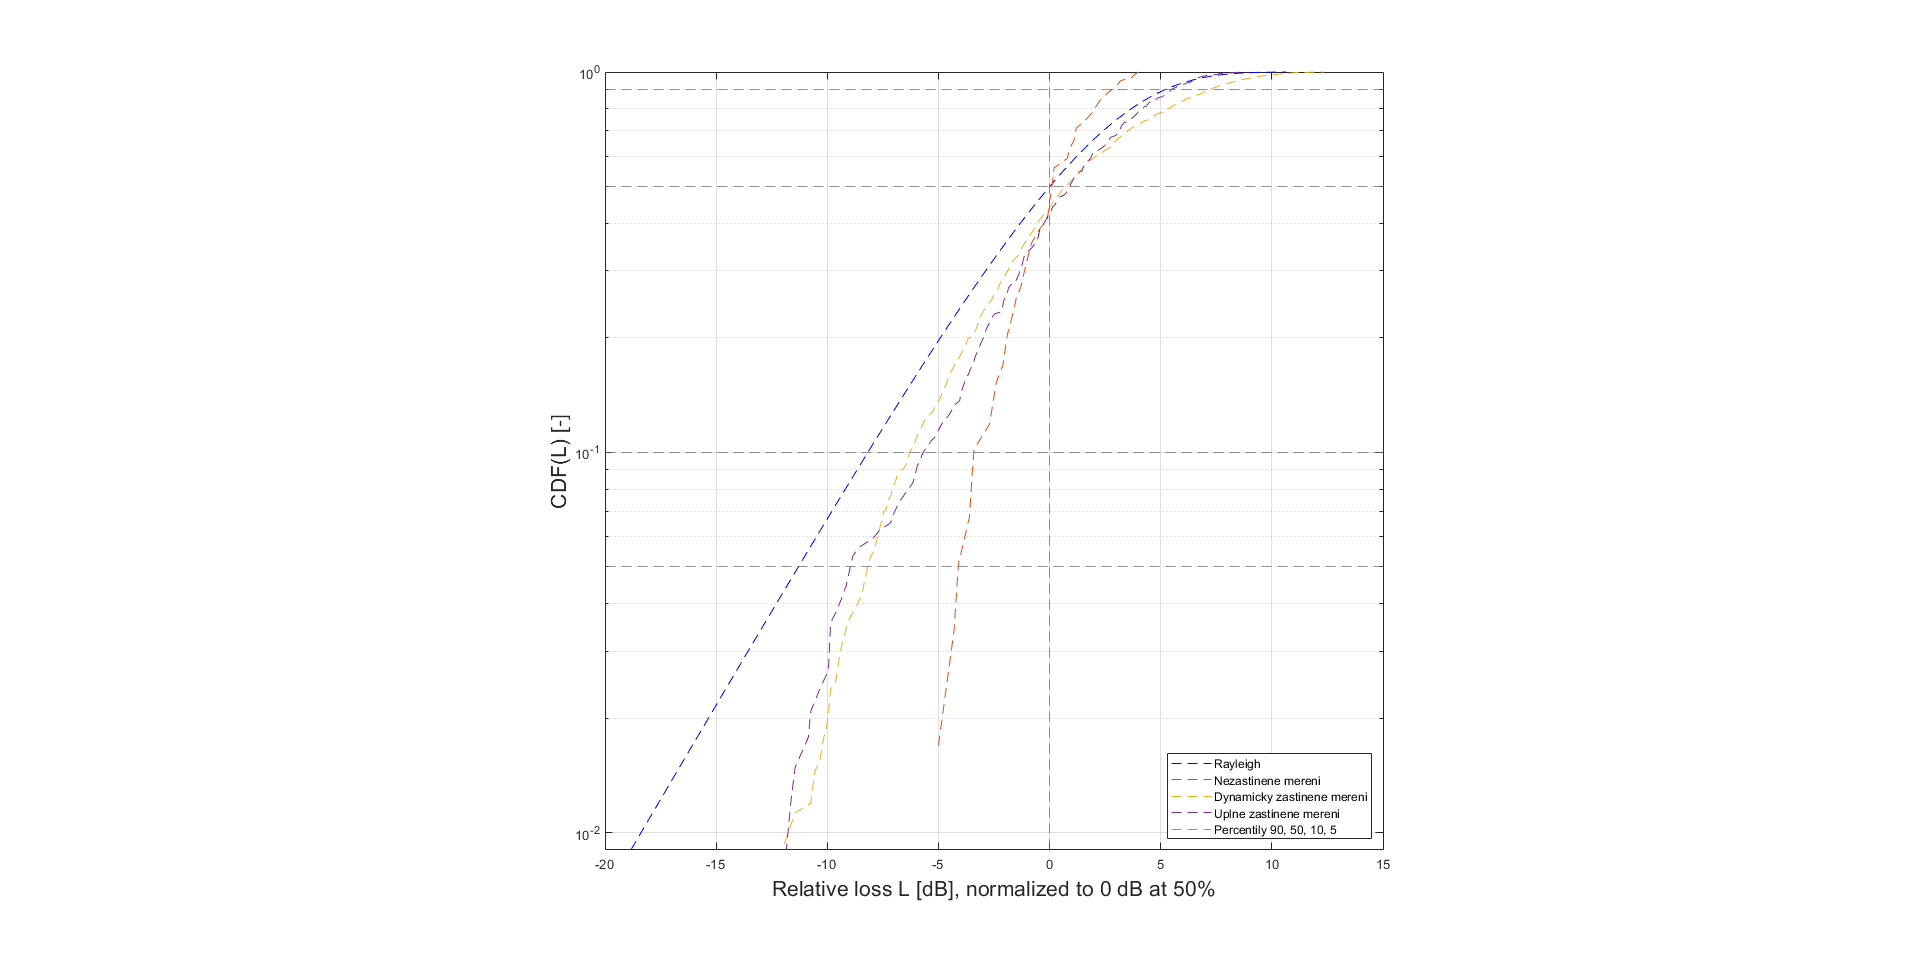
\includegraphics[width=.45\textwidth]{src/uniky-rayleigh.png}
	\end{figure}
\end{frame}

\section{Závěr}
\begin{frame}{Závěr - Jugoslávských partyzánů}
	\begin{figure}[!ht]
		\centering
		\begin{subfigure}[b]{.45\textwidth}
			\centering
			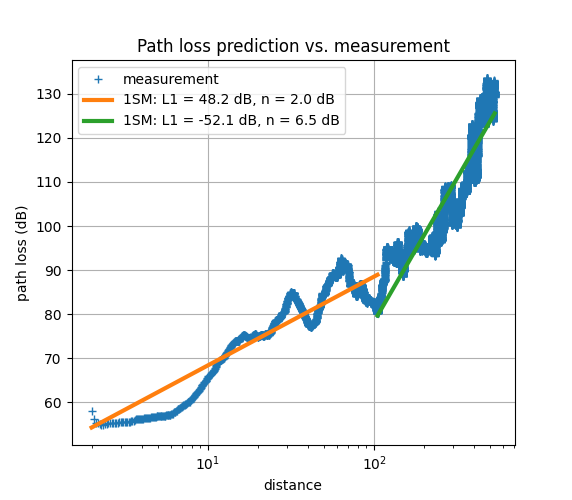
\includegraphics[width=\textwidth]{src/partyzanu-od-vysilace-4.png}
		\end{subfigure}
		\begin{subfigure}[b]{.45\textwidth}
			\centering
			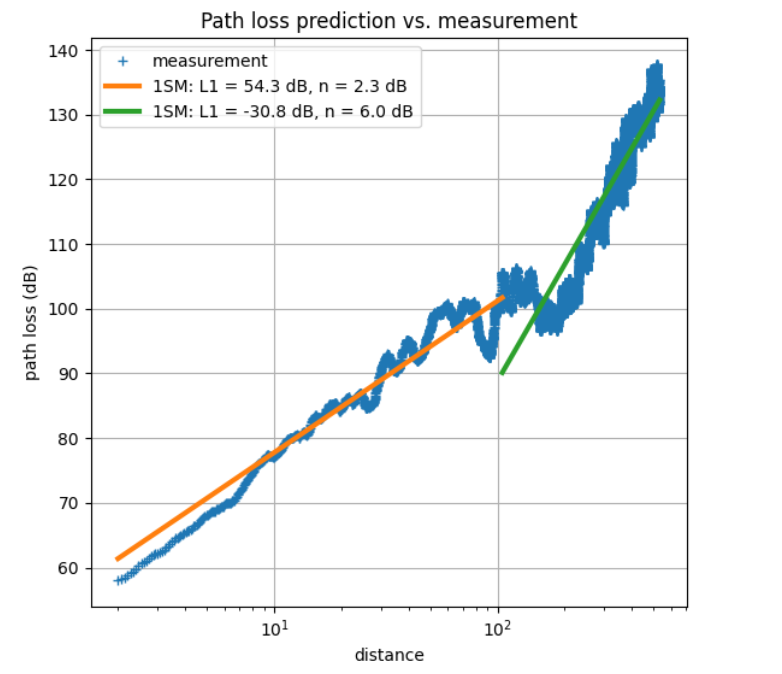
\includegraphics[width=\textwidth]{src/partyzanu-k-vysilaci-4.png}
		\end{subfigure}
	\end{figure}
\end{frame}
\begin{frame}{Závěr - Rayleigh fading}
	\begin{figure}[!ht]
		\centering
		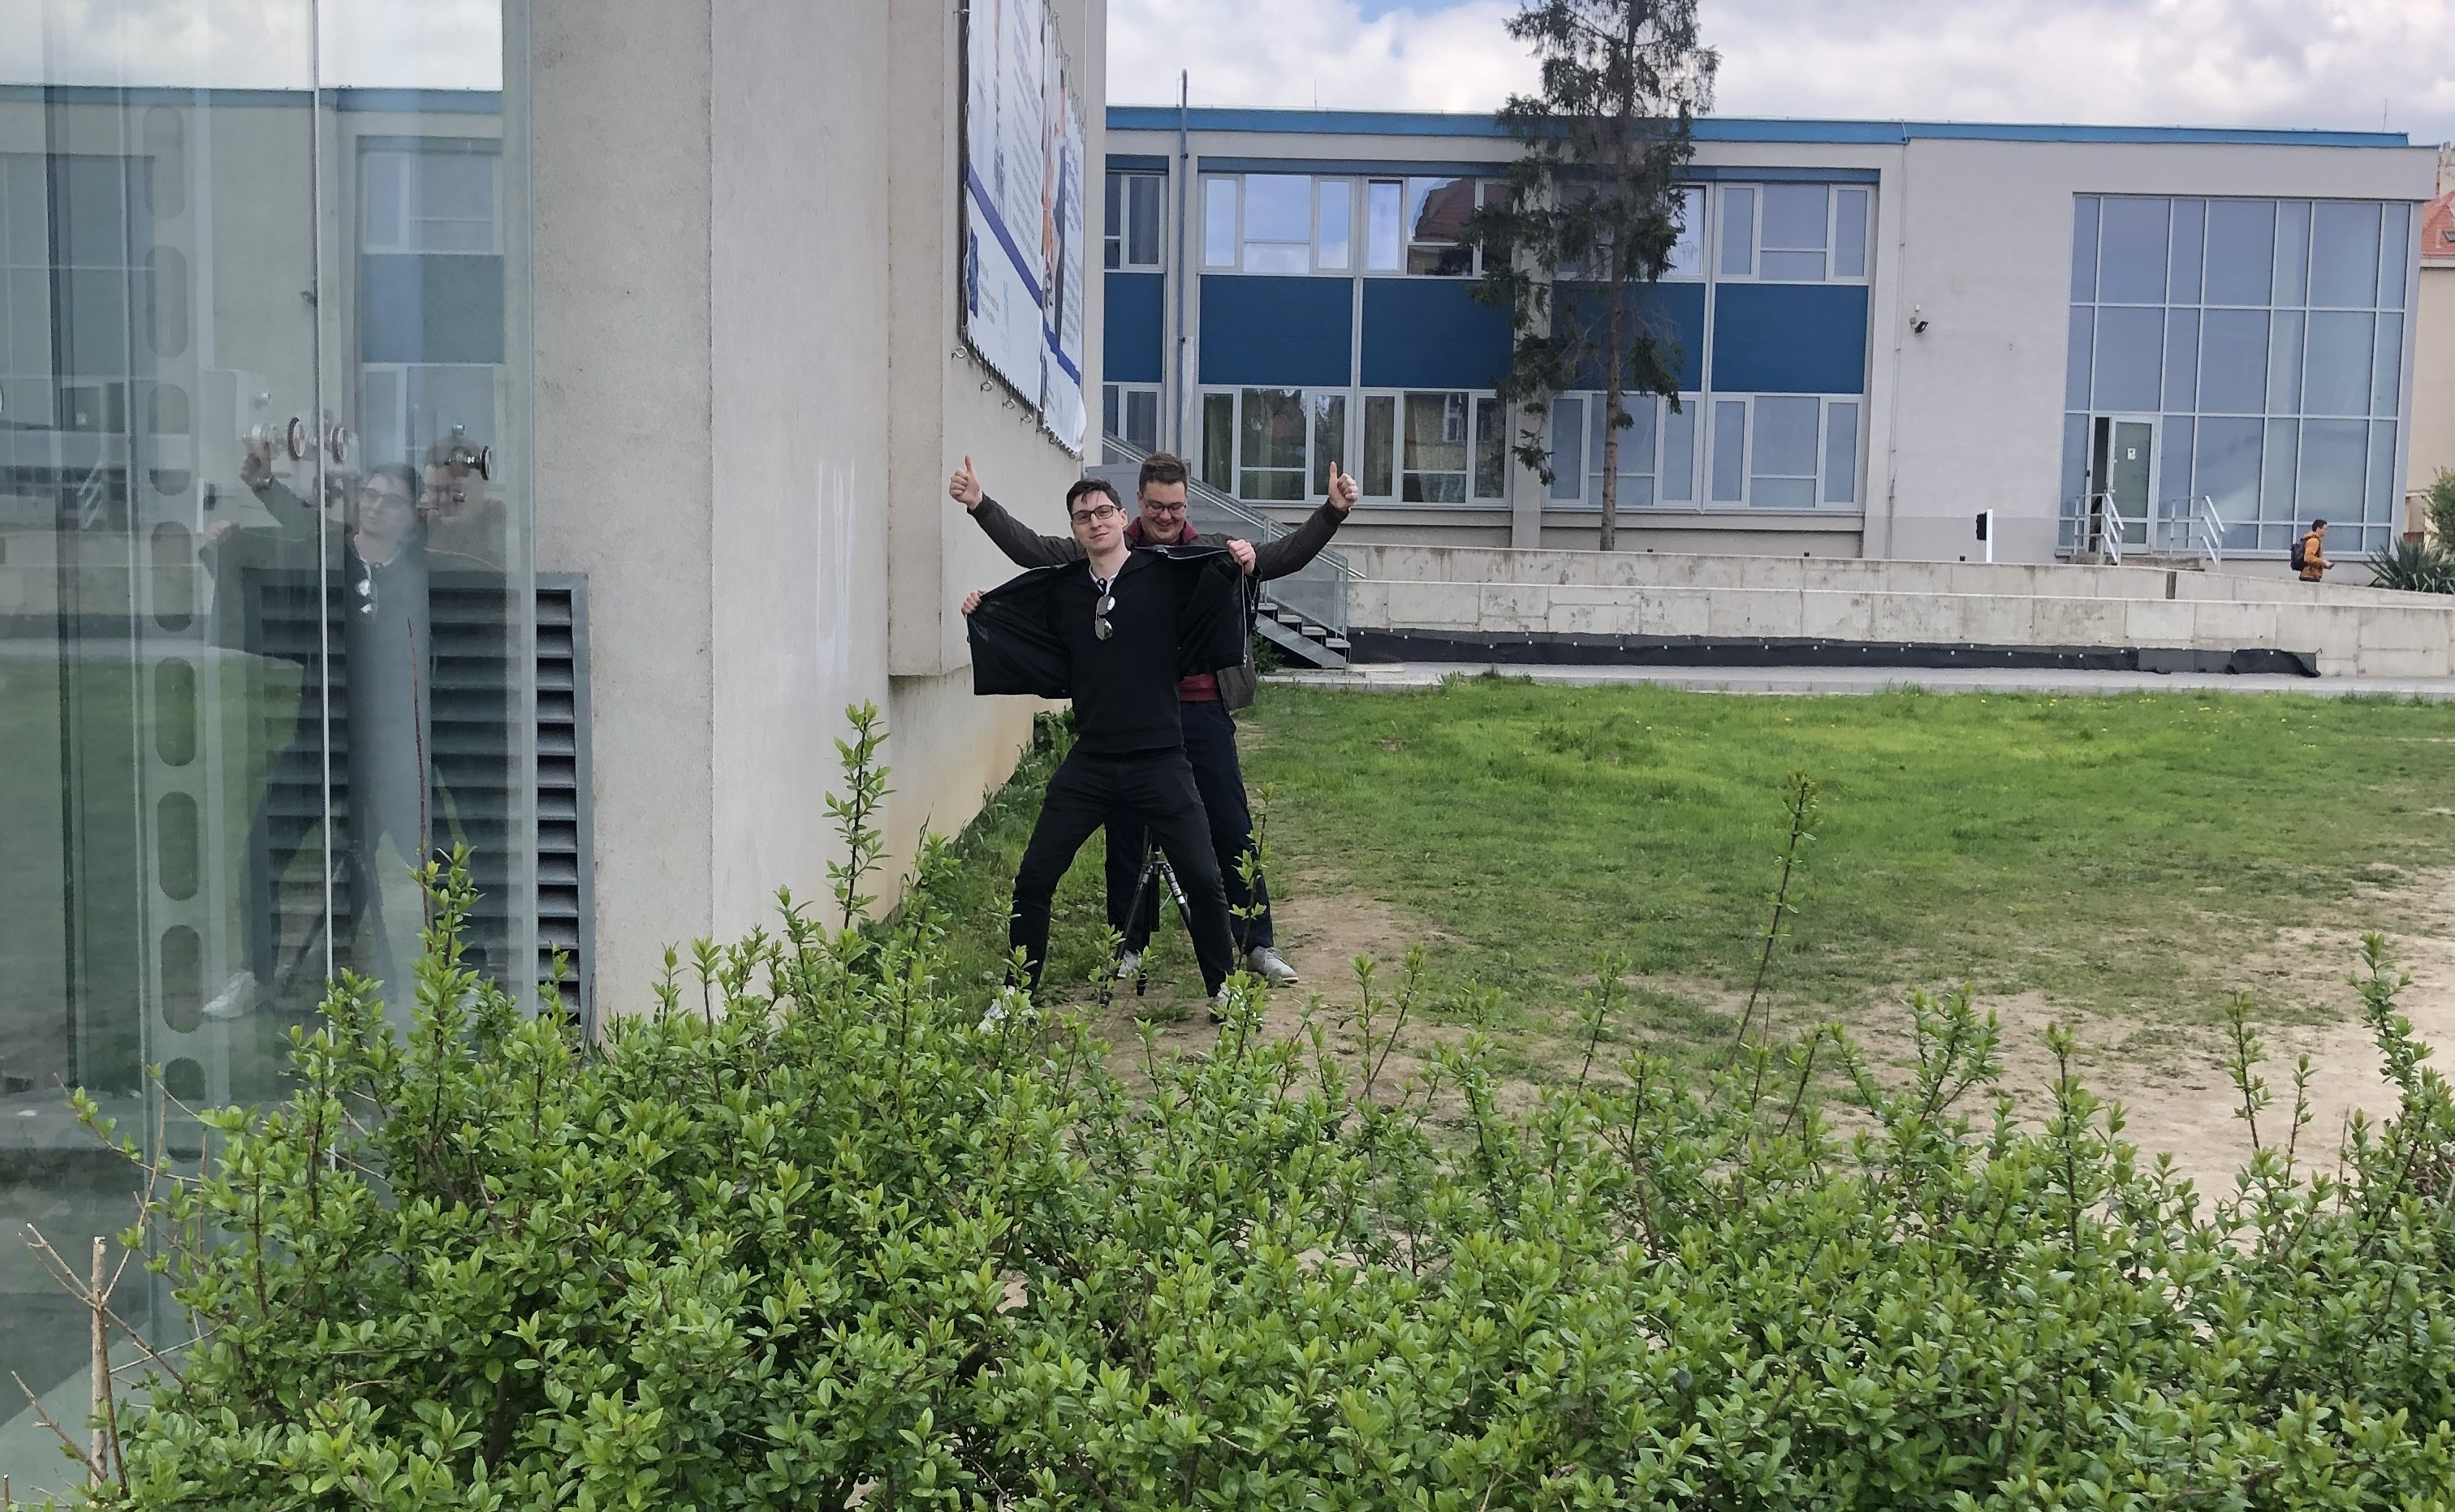
\includegraphics[width=.7\textwidth]{src/fotka-rayleigh.jpg}
	\end{figure}
\end{frame}

\setbeamercolor{background canvas}{bg=white}

\end{document}
